% IEEE Access draft (third paper). Compile with the official IEEE Access LaTeX template
% (ieeeaccess.cls, spotcolor.sty, IEEEtran.bst, logo files) copied into this directory; see paper3/README.md.
% Status: skeleton. Plan: docs/paper3_5g_multicell_plan.md. Every section is outlined with \todo{...}.
\documentclass{ieeeaccess}
\usepackage{cite}
\usepackage{amsmath,amssymb,amsfonts}
\usepackage[ruled,linesnumbered]{algorithm2e}
\usepackage{graphicx}
\usepackage{textcomp}
\usepackage{booktabs}
\usepackage{xcolor}
\graphicspath{{figures/}}
\newcommand{\todo}[1]{\textcolor{red}{[TODO: #1]}}

\begin{document}
\history{Date of publication xxxx 00, 0000, date of current version xxxx 00, 0000.}
\doi{10.1109/ACCESS.2026.0000000}

\title{When Does Multi-Cell Coordination Pay Off? An Exact-Oracle Gap Analysis of Learned Schedulers in 5G NR}
\author{\uppercase{Pyoungyun Kim}\authorrefmark{1,2}, \IEEEmembership{Student Member, IEEE}, and \uppercase{Taeyoon Kim}\authorrefmark{3}}
\address[1]{Korea University, 145 Anam-ro, Seongbuk-gu, Seoul 02841, Republic of Korea}
\address[2]{Visual Display Division, Samsung Electronics, Republic of Korea}
\address[3]{School of Mobile System Engineering, Dankook University, Yongin 16890, Republic of Korea}
% Funding statement: none yet. Add \tfootnote{This work was supported by ...} when available.

\markboth
{P. Kim \emph{et al.}: Exact-Oracle Gap Analysis of Learned Multi-Cell Schedulers in 5G NR}
{P. Kim \emph{et al.}: Exact-Oracle Gap Analysis of Learned Multi-Cell Schedulers in 5G NR}

\corresp{Corresponding author: Taeyoon Kim (e-mail: 2000kty@dankook.ac.kr).}

\begin{abstract}
Coordinated scheduling across cells in fifth-generation new radio (5G NR) decides in every slot which cell serves which user equipment (UE) on each subband and which cells stay silent. Learned schedulers based on multi-agent reinforcement learning (MARL) with centralized training and decentralized execution (CTDE) fit the open radio access network (O-RAN) architecture, in which a near-real-time radio access network intelligent controller (near-RT RIC) trains centrally and each base station executes locally. Their gains are, however, measured against heuristics whose distance from the optimum is unknown. This paper computes an exact per-slot oracle for coordinated scheduling, decomposes the loss of learned schedulers relative to it, and identifies the operating conditions under which coordination beyond a time-division reference yields a gain. \todo{Main quantitative results: headroom versus offered load relative to the capacity of cluster time division, share of the variance explained by the fluid model, link-adaptation, information, and optimization gaps with outer-loop link adaptation, and their dependence on channel quality indicator delay and UE speed.}
\end{abstract}

\begin{keywords}
5G NR, coordinated scheduling, inter-cell interference coordination, multi-agent reinforcement learning, centralized training with decentralized execution, O-RAN, link adaptation.
\end{keywords}

\titlepgskip=-21pt

\maketitle

\section{Introduction}
\label{sec:introduction}
\PARstart{D}{ense} deployments of fifth-generation new radio (5G NR) base stations operate with full frequency reuse, so that the throughput of a cell depends on the scheduling decisions of its neighbors. Coordinated scheduling lets a cluster of cells decide jointly which user equipment (UE) each cell serves on each subband and which cells stay silent. The open radio access network (O-RAN) architecture places such decisions in a near-real-time radio access network intelligent controller (near-RT RIC), which makes multi-agent reinforcement learning (MARL) with centralized training and decentralized execution (CTDE)~\cite{lowe2017maddpg,foerster2018coma,yu2022mappo} a natural fit: the controller trains a centralized critic, and each base station executes a local actor.

\todo{Gap in evaluation practice: learned coordinated schedulers are compared with uncoordinated proportional fair (PF) scheduling or static reuse, neither of which is an upper bound. Summary of the companion IEEE 802.11bn study and the open question whether its findings are specific to Wi-Fi.}

\todo{Contributions: (i) exact per-subband oracle for coordinated scheduling under full buffer, (ii) headroom law with respect to cluster time division and a fluid model, (iii) loss decomposition with outer-loop link adaptation (OLLA) as the standard link adaptation, (iv) dependence on channel quality indicator (CQI) delay, UE speed, PF objective, and cluster size, (v) reproducible simulator.}

\todo{Organization paragraph: the only place in Section~\ref{sec:introduction} that names later sections.}

\section{Related Work}
\label{sec:related}
\subsection{Coordinated scheduling and interference coordination}
\todo{Coordinated multipoint (CoMP) coordinated scheduling and beamforming, enhanced inter-cell interference coordination (eICIC), fractional frequency reuse. Every citation verified against a primary record before it enters references.bib.}

\subsection{Learning-based scheduling in cellular networks}
\todo{MARL for inter-cell interference coordination and power control; reinforcement learning xApps in O-RAN; optimality references used in these studies.}

\section{System Model}
\label{sec:system}
\subsection{Layout and coordination cluster}
\todo{Hexagonal layout of seven cells with wraparound and inter-site distance (ISD) of 200~m; coordination cluster $\mathcal{C}$ of size $C \in \{3, 7\}$; cells outside $\mathcal{C}$ transmit with uncoordinated PF scheduling and act as background interference; $U$ UEs per cell dropped uniformly with a minimum distance of 10~m.}

\begin{figure*}
\centering
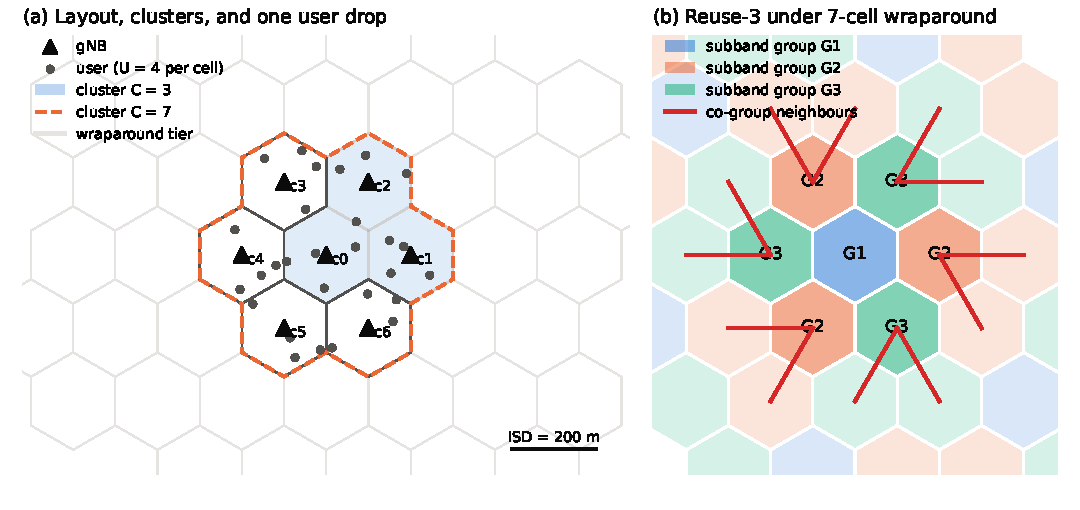
\includegraphics[width=\textwidth]{paper3_topology}
\caption{Layout and orthogonal reference. (a) Seven-cell hexagonal layout with its wraparound tier, the coordination clusters $C = 3$ and $C = 7$, and one drop of $U = 4$ UEs per cell. (b) Location-based reuse-3 under a seven-cell wraparound, where co-group cells meet across the wrap boundary; the orthogonal reference is therefore cluster time division.}
\label{fig:topology}
\end{figure*}

\subsection{Channel}
\todo{Simplified 3GPP TR 38.901 urban micro (UMi) path loss with line-of-sight probability, log-normal shadowing, subband Rayleigh fading with Gauss--Markov time correlation $\rho = J_0(2\pi f_D T_{\text{slot}})$. Parameter values verified against TR 38.901.}

\subsection{Resources, actions, and link outcome}
\todo{Slot duration $T_{\text{slot}}$, $B$ subbands, per-subband target UE or silence of every cell, CQI table of TS 38.214 with signal-to-interference-plus-noise ratio (SINR) thresholds, step block error model.}

\subsection{Traffic and objective}
\todo{Full buffer and finite buffer; slot throughput and PF objective with exponentially averaged rates.}

\subsection{Observations}
\todo{Delayed per-subband CQI, buffer length, PF average rate, mean interference from neighboring cells; information level $b \in \{0, \infty\}$.}

\section{Problem Formulation}
\label{sec:problem}
\todo{Per-slot objective, episode objective, decentralized partially observable Markov decision process~\cite{oliehoek2016dec}; offered load relative to the capacity of cluster time division, $\rho$.}

\section{Exact Oracle, References, and Learners}
\label{sec:method}
\subsection{Exact per-subband oracle}
\todo{Separability across subbands under full buffer; enumeration of $(U+1)^C$ joint decisions per subband with the highest decodable modulation and coding scheme (MCS) per link; runtime; Algorithm in algorithm2e style.}

\subsection{Reference schedulers}
\todo{Uncoordinated reuse-1 PF, cluster time division, greedy muting, and the better of the three per drop.}

\subsection{Learned schedulers and gap decomposition}
\todo{MAPPO~\cite{yu2022mappo} and Central PPO trained with PPO~\cite{schulman2017ppo} and generalized advantage estimation~\cite{schulman2016gae}; one agent per cell and subband with shared parameters; MCS control learned, OLLA, or ideal; link-adaptation, information, and optimization gaps.}

\section{Experimental Setup}
\label{sec:setup}
\todo{Experiments E0--E5 of the plan: calibration, headroom sweep over drops, loss decomposition, CQI delay and UE speed, PF versus throughput objective, cluster size.}

\section{Results}
\label{sec:results}
\todo{Results.}

\section{Discussion}
\label{sec:discussion}
\todo{Comparison with the IEEE 802.11bn findings; design guidance; limitations.}

\section{Conclusion}
\label{sec:conclusion}
\todo{Conclusion.}

% Acknowledgment: none yet. Add \section*{Acknowledgment} here when available.

\bibliographystyle{IEEEtran}
\bibliography{references}

\begin{biography}[{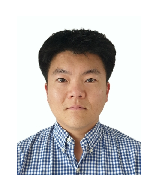
\includegraphics[width=1in,height=1.25in,clip,keepaspectratio]{photo/kpy.eps}}]{Pyoungyun Kim} (S'25)
received the B.S. and M.S. degrees from Korea University, Seoul, Korea, in 2005 and 2007, respectively. Since 2007, he has been with Samsung Electronics, where he has contributed to smart recommendation agents, the integration of the Consumer Electronics Control (CEC) protocol into television systems, and Tizen-based TV software applications. He is currently a Senior Engineer with the Product S/W Lab, Visual Display Division, Samsung Electronics, where he works on multi-view features for smart TVs and screen control for projectors. His research interests include on-device artificial intelligence (AI) for smart displays, embedded deep learning optimization, and resource-efficient deep reinforcement learning (DRL).
\end{biography}

\begin{biography}[{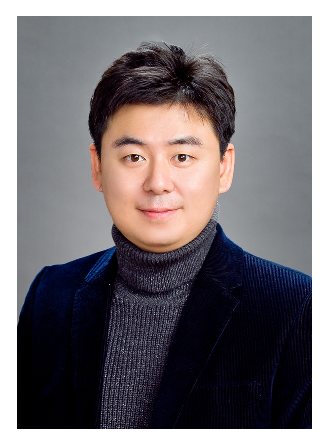
\includegraphics[width=1in,height=1.25in,clip,keepaspectratio]{photo/kty.eps}}]{Taeyoon Kim}
received the B.S., M.S., and Ph.D. degrees in electronics and computer engineering from Korea University in 2005, 2007, and 2019, respectively. He was a Research Engineer with Hyundai Motors from 2007 to 2010 and an Assistant Professor with Soonchunhyang University from 2019 to 2021. In 2021, he joined Dankook University as an Assistant Professor with the School of Mobile System Engineering. He was a Visiting Researcher with the University of British Columbia in 2017. His research interests include network architectures and protocols for next-generation networks, such as WLAN, 5G, and time-sensitive networking (TSN), and AI-enabled edge intelligence.
\end{biography}

\EOD

\end{document}
